\documentclass[reprint, amsmath,amssymb, aps,pra]{revtex4-1}

\usepackage[utf8]{inputenc}
\usepackage[draft,inline,nomargin]{fixme}
\usepackage{graphicx}
\usepackage{dcolumn}
\usepackage{bm}
\usepackage{braket}
\usepackage{physics}






\begin{document}

%\preprint{APS/123-QED}

\title{Cooling in a parametrically driven optomechanical cavity}%

\author{Pablo Yanes-Thomas}

\author{Marc Bienert}

\author{Pablo Barberis-Blostein}

\affiliation{Instituto de Investigaciones en Matem\'{a}ticas Aplicadas y en Sistemas,
Universidad Nacional Aut\'{o}noma de M\'{e}xico, Circuito Escolar s/n Ciudad Universitaria M\'{e}xico, D.F.}%



\date{\today}

\begin{abstract}

  We obtain a master equation for a parametrically driven
  optomechanical cavity using a dissipation model that accounts for
  the modification of the quasi-energy spectrum caused by the driving
  when the natural frequency of the mechanical object oscillates
  periodically around its mean value. The master equation with its
  improved dissipation model is expressed using Floquet operators. We
  apply the master equation to model the laser cooling of the
  mechanical object. Using an adiabatic approximation, an analytical
  expression for its temperature can be obtained. This expression
  depends both on the oscillator's mean frequency and that of the
  frequency's oscillations around its mean value. We find that the
  temperature can be lower than in the non-time dependent case. Our
  results raise the possibility of achieving lower temperatures for
  the mechanical object if its natural frequency can be controlled as
  a function of time.
\end{abstract}

\pacs{Valid PACS appear here}% PACS, the Physics and Astronomy
                             % Classification Scheme.
%\keywords{Suggested keywords}%Use showkeys class option if keyword
                              %display desired
\maketitle

%\tableofcontents

\section{Introduction}


Quantum cavity optomechanics studies systems composed of macroscopic
mechanical objects, such as mirrors, and an optical cavity's quantized
light field usually coupled via radiation pressure. In a common scheme
one of the end-mirrors of a Fabry-Perot cavity is suspended while able
to freely oscillate. When photons are reflected by the mirror, there
is a momentum transfer between the light field and the mirror and
hence a coupling force. As the cavity's resonance depends on its
length, the mechanical displacement in turn affects the light field
inside the cavity. Some of the first theoretical work predicting this
sort of coupling is described in \cite{BraginskiiOG}. This interaction
between the macroscopic mechanical object and the light field leads to
several interesting effects such as optomechanically induced
transparency \cite{WeissOIT}, the optical spring effect \cite{VogelOT}
or, most relevant to this study, optomechanical cooling, which was
first proposed by Mancini, et al \cite{CohadonCM, CorbittOC,
  SchliesserRPC, LCNooshi, ManciniOC}.
	
Optomechanical cooling consists of the damping of the end mirror's
mechanical motion due to the radiative coupling to the cavity field.
Sideband cooling takes place when the cavity's resonance is much
narrower than the mechanical frequency. It can be understood as Raman
scattering of incident photons \cite{MarquardtQTOQ} which are
red-detuned from the cavity resonance. When the parameters are chosen
appropriately, incident photons must absorb a phonon from the
mechanical oscillator in order to scatter into the cavity's resonance
mode, resulting in cooling of the resonator. For coherent quantum
control over a mechanical object, it must be close to a pure quantum
mechanical state \cite{KippenberCO} so effective methods of cooling
macroscopic objects to low temperatures are highly desirable.

One possible avenue for manipulating the mechanical object and
improving cooling lies in controlling the mechanical resonator's
frequency as a function of time \cite{JockelMR}. The effect of this
dependence on the mechanical object's final temperature was studied in
\cite{BarberisLC}. In that study it was found that the final
temperature of the parametrically driven harmonic oscillator was
larger than the nondriven case. However, the master equation from
which the cooling rates were derived accounted for the natural
frequency of the mechanical resonator via ad-hoc time-dependent
coefficients that were introduced after performing the Markov
approximation; this approach led to an incomplete master equation and
thus an incomplete description of the system's dynamics, as the system
is being treated as essentially not time-dependent during the
derivation of the master equation. In this study, we employ a
different method that accounts for the time dependence throughout the
entire derivation.


The formalism we apply (section \ref{OptmechH}) is based on
Floquet theory and was demonstrated to be a more accurate treatment in
\cite{HanngiFM}. For the case where the drive consists of a small
periodic oscillation with respect to the central frequency of the
mechanical oscillator, the Floquet operators can be given explicitly
(section \ref{SolSmallOsc}). Under the adiabatic approximation, we
derive an approximated expression for the mean phonon occupation
number in the final stages of optomechanical cooling (section
\ref{LasCool}), and compare its prediction to the non-time-dependent
case (section \ref{NumCal}). We find, using the formalism presented
here, that lower temperatures can be obtained if the mechanical object
is parametrically driven. Our results suggest that the theoretical
model of dissipation of the mechanical osscilator can have a
significant influence on the resulting temperature (section
\ref{ConCl}).


% The formalism which we apply is based on Floquet theory and was
% demonstrated to be a more accurate treatment in \cite{HanngiFM}. We
% obtain a master equation expressed in terms of Floquet operators and
% from there derive an approximated expression for the final mechanical
% state's mean phonon occupation number, which is used as a proxy for
% the state's temperature, under the adiabatic approximation. We perform
% numerical calculations in order to compare this expression to the one
% for the non-time-dependent case.

%We study the cooling of a macroscopic mechanical harmonic oscillator
%with time-dependent natural frequency coupled to an optical cavity's
%light field via radiation pressure when the mechanical oscillator's
%natural frequency varies periodically in time with a small amplitude
%vis-a-vis a constant central frequency. Typically \cite{BarberisLC},
%the interaction between the two systems is too small for the cooling
%to be faster than the system's re-thermalization, so a laser, which
%acts as a photon pump, is employed to boost the interaction.

% The paper is structured as follows. In section \ref{OptmechH}, a
% Hamiltonian for optomechanical cooling for the time-dependent harmonic
% oscillator is presented and expressed in terms of time-dependent
% operators and in a displaced reference frame. In section
% \ref{SolSmallOsc}, we calculate explicit expressions  for the specific case of small periodic oscillations. The
% corresponding master equation is obtained in terms of these explicit
% expressions under the Markov approximation. In section
% \ref{LasCool}, we derive a master equation under the adiabatic
% approximation for only the mechanical degrees of freedom and obtain an
% explicit expression of the mean vibrational occupation number as a
% measure of the final state's temperature. Finally, we compare the
% temperature prediction for the non-time dependent case to the new
% prediction obtained in this study.

\section{Optomechanical Hamiltonian}\label{OptmechH}
\subsection{Hamiltonian with Floquet Operators}
	
The Hamiltonian for a parametrically driven optomechanical system
\cite{LCNooshi}, in a reference system that rotates with the same
frequency as a laser that continuously pumps photons into the cavity
is

\begin{equation}
H(t) =   H_{\rm cav} + H_{\rm mec}(t) + H_{\rm int} + H_{\rm pump},
\end{equation}

where

\begin{align}
H_{\rm cav} =& -\hbar \delta a^\dagger a,\\
H_{\rm mec}(t) =& \frac{p^2}{2M} + \frac{1}{2}M \nu^2 (t) x^2,\\
H_{\rm int} =& -\hbar g a^\dagger a x,\\
H_{\rm pump} =& \hbar\frac{\Omega}{2}(a^\dagger + a),
\end{align}
Where $\delta = \omega_{laser} - \omega_{cav}$, in the cavity Hamiltonian, $H_{\rm cav}$, is the frequency difference between the laser and
the cavity; $M$, in the mechanical oscillator Hamiltonian,
$H_{\rm mec}$, is the mechanical oscillator's mass, $p$ its momentum
operator, $x$ its position operator, and $\nu(t)$ its frequency. The
$H_{\rm int}$ term models the interaction between the field and the cavity
mirror where $g$ sets the strength of the coupling \cite{KippenberCO}.
Finally, $H_{\rm pump}$ describes the pumping of the cavity by a field with
a strength proportional to $\Omega$. The mechanical oscillator Hamiltonian has an explicit time dependence given by
$\nu(t)$; in order to employ the Floquet formalism this dependence must be a
periodic function of time.

The Floquet operators are analogous to the usual creation and
annihilation operators for the standard harmonic oscillator and can be
expressed in terms of the mechanical oscillator's position and
momentum operators \cite{HanngiFM}. These operators are

\begin{equation}\label{FloquetOperators}
\Gamma(t) = \frac{1}{2i}\left[\hat{x}\sqrt{\frac{2M}{\hbar}}\dot{f}(t)-\hat{p}\sqrt{\frac{2}{M \hbar }}f(t)\right],
\end{equation} as well as its Hermitian conjugate. $f(t)$ is the solution to the classical time-dependent harmonic oscillator equation of motion in one dimension 

\begin{equation} \label{TimeDependentHO}
\ddot{f} + \nu(t)^2f=0,
\end{equation} and is generally a complex function \cite{BrownPT}. This equation has two solutions \cite{HanngiFM} 
\begin{equation}
f(t) = e^{i\mu t}\phi(t), 
\end{equation}
and its complex conjugate, where $\phi(t)$ is a periodic function of
time with the same period as $\nu(t)$. $\mu$ is, in general, a complex
number \cite{WardFT}. The Floquet operators follow the usual
commutation relations for creation and annihilation operators
\begin{equation}
[\Gamma(t)^\dagger,\Gamma(t)]=1.
\end{equation}

 Using these operators $H_{\rm mec}(t)$ can be written in the same form as the non time-dependent harmonic oscillator with the Floquet operators taking the place of the annihilation operators, with the exception of a global time-dependent scalar coefficient  \cite{BrownPT}

\begin{equation}
H_{\rm mec}(t) = \hbar\frac{W}{|f(t)|^2}\left[\Gamma^\dagger(t)\Gamma(t) + \frac{1}{2}\right],
\end{equation}
with the Wronskian $W$ for \eqref{TimeDependentHO}. The explicit time dependence of the Floquet operators will not be noted from now on for the sake of brevity. Equation
\eqref{FloquetOperators} is inverted and solved for the harmonic
oscillator's position operator \cite{TesisMaestria}

\begin{equation}
\hat{x} = \frac{b^* \Gamma - b\Gamma^\dagger}{(b^*c-bc^*)}
\end{equation} with

\begin{align}
c =&  \frac{1}{2i}\sqrt{\frac{2M}{\hbar}}\dot{f}\, , \\
b =&  \frac{1}{2i}\sqrt{\frac{2}{M\hbar}}f\, .
\end{align}
These are then substituted back into the interaction Hamiltonian
resulting in

\begin{equation}
H_{\rm int}(t) = g\sqrt{\frac{\hbar}{2M}}a^\dagger a[\gamma_+(t)\Gamma +\gamma_-(t)\Gamma^\dagger],
\end{equation} with coefficients

\begin{align*}
\gamma_+(t)=&\frac{f^*}{(f^*\dot{f}-f\dot{f}^*)},\\
\gamma_-(t)=&\frac{f}{(f\dot{f}^*-f^*\dot{f})}\, .
\end{align*} 


The Hamiltonian contains two separate harmonic oscillator-like terms
that commute with each other, $H_{\rm cav}$ and $H_{\rm mec}$, so the
standard harmonic oscillator master equation structure can be derived
\cite{TesisMaestria}\cite{HanngiFM}. The usual derivation of the
master equation involves a Markov approximation; in previous attempts
to study this type of system, the time dependence of the frequency was
included after the Markov approximation had been performed, via
time-dependent ad-hoc coefficients for the damping \cite{BarberisLC}.
We use the formalism developed in \cite{HanngiFM} to derive the
mechanical dissipation of the optomechanical master equation. Under
this formalism, the frequency's time dependence is accounted for when the
Markov approximation is performed, via the Floquet operators. As
demonstrated in \cite{HanngiFM}, the method employed here is a more
complete, and thus accurate, treatment.

The optomechanical master equation with improved dissipation model is
\begin{equation} \label{LCMasterEquation}
\dot{\rho} = \frac{1}{i\hbar}[H,\rho] +L_a\rho + L_\Gamma \rho,
\end{equation}
where
\begin{align}
L_a \rho =& - \frac{\kappa}{2}(n_p + 1)[a^\dagger a\rho + \rho a^\dagger a -2a\rho a^\dagger]  \\
 &- \frac{\kappa}{2}(n_p)[ aa^\dagger\rho + \rho  aa^\dagger -2a^\dagger\rho a]\, ,\nonumber
\end{align}

\begin{align}\label{eq:mechanical_dissipation}
  L_\Gamma \rho =& - \frac{\gamma}{2}(n_m + 1)[\Gamma^\dagger \Gamma\rho + \rho \Gamma^\dagger \Gamma -2\Gamma\rho \Gamma^\dagger]  \\
                 &- \frac{\gamma}{2}(n_m)[ \Gamma\Gamma^\dagger\rho + \rho  \Gamma\Gamma^\dagger -2\Gamma^\dagger\rho \Gamma]\, ,\nonumber
\end{align} 
$\kappa$ is the energy decay rate for the cavity and $\gamma$ is the
decay rate for the mechanical oscillator. The number of thermal
excitations for the cavity and the oscillator are given by $n_p$ and
$n_m$ respectively. The superoperators $L_\Gamma$ and $L_a$ model the
energy exchanges between the environment, and the cavity and the
mechanical resonator respectively. Equation \eqref{LCMasterEquation}
is the master equation for a parametrically driven optomechanical
system with an improved dissipation model which accounts for the
mechanical oscillator's time dependent frequency.



\subsection{Displaced Frame}

In order to eliminate the pump term and to find useful approximations
we employ a unitary transformation to shift \eqref{LCMasterEquation}
into a displaced reference frame. This transformation depends on two
time-dependent coefficients, $\alpha(t)$ and $\beta(t)$, which are
chosen in a convenient manner to simplify the Hamiltonian. The
transformation is given by the operator
\begin{equation}\label{ShiftTransform}
U_{a,\Gamma} = e^{(\alpha(t) a^\dagger - \alpha^*(t)a)}e^{(\beta(t) \Gamma^\dagger - \beta^*(t)\Gamma)},
\end{equation}
and results in a displaced Hamiltonian and in turn a displaced master
equation
\begin{equation}\label{eq:master_no_small}
\dot{\rho}' = \frac{1}{i\hbar}[H',\rho'] +L_a\rho' + L_\Gamma \rho' + C(t)\rho' ,
\end{equation} for the time evolution of the density operator
$\rho'(t)=U\rho U^\dagger$ which represents the coupled
cavity-mechanical system,  with 

\begin{equation}
C(t)=(\beta^2-|\beta|^2)[\dot{\Gamma}^\dagger,\Gamma^\dagger]-((\beta^*)^2-|\beta|^2)[\dot{\Gamma},\Gamma].
\end{equation}
The primes indicate that the transformation has been applied. The
displaced Hamiltonian, which includes a pump-like term that appears
due to the transformation being applied to the time derivative term,
is
\begin{align}\label{eq:hamiltonian_no_small}
  H'=&U H U^\dagger\nonumber\\=& -\hbar \delta' a^\dagger a + \hbar\frac{W}{|f(t)|^2}\Gamma \Gamma^\dagger\nonumber\\
     &-\hbar g\sqrt{\frac{\hbar}{2M}}[(a^{\dagger}a +\alpha a^{\dagger}+\alpha^* a)(\gamma_-(t)\Gamma^{\dagger}+\gamma_+(t)\Gamma)]\nonumber\\
     &+ i\hbar(\beta^*\dot{\Gamma} - \beta \dot{\Gamma}^\dagger),
\end{align}
with $\delta' = \delta + g\sqrt{\frac{\hbar}{2M}}(\gamma_+(t)\beta + \gamma_-(t)\beta^*)$.
This Hamiltonian is valid as long as the coefficients $\alpha(t)$ and
$\beta(t)$ fulfill the differential equations

\begin{align}\label{eq:displaced_frame}
\dot{\alpha} =& \alpha(-\frac{\kappa}{2}+i(\delta+g\sqrt{\frac{\hbar}{2M}}(\gamma_-(t) \beta^* + \gamma_+(t) \beta))-i\frac{\Omega}{2},\\
\dot{\beta} =& \beta(-\frac{\gamma}{2}-i\frac{W}{|f(t)|^2})+ig\sqrt{\frac{\hbar}{2M}}|\alpha|^2\gamma_+(t).
\end{align}


The $C(t)$ term appears because the Floquet operators do not necessarily commute with
their own time derivatives.

Proceeding further requires an explicit solution for
\eqref{TimeDependentHO} in order to calculate explicit expressions for several of the coefficients and to deal with the $\dot{\Gamma}$ and $\dot{\Gamma}^\dagger$ operators. The primes in the operators will be omitted
from now on as all calculations will carried out in the displaced frame.


\section{Solution for Small Oscillations}\label{SolSmallOsc}
 
In order to obtain an explicit form of the Floquet operators we focus
on the case of small oscillations around a central frequency,
specifically

\begin{equation}
\nu(t) = \nu_0 + \epsilon' cos(2\omega t)\, ,
\end{equation}
with $\epsilon' \ll \nu_0$, where $\nu_0$ is the mean frequency. This
leads to the time-dependent harmonic oscillator equation

\begin{equation}\label{SmallOscillationsTDHO}
\ddot{f} + (\nu_0^2 + 2\epsilon' \nu_0 cos(2\omega t))f = 0,
\end{equation}
which is a particular case of the Mathieu equation \cite{PiatekME}.
In order to guarantee stable solutions we require the scattering
relation
\begin{equation}
\frac{\nu_0^2}{\omega^2} = n^2,\label{scattering}
\end{equation}
with $n \in \mathbb{Z}^+$\cite{WardFT}. We will focus on the case
$n\gg 1$, which will be used in the next sections. The solutions for
\eqref{SmallOscillationsTDHO} are, to first order in
$\epsilon= \frac{2\epsilon' \nu_0}{\omega^2}$,
\begin{equation}\label{SmallOscillationsSolution}
f(t)=  \frac{1}{\sqrt{n\omega}}(e^{in\omega t}  + \epsilon \frac{1}{8(n+1)} e^{i(n+2) \omega t} - \epsilon \frac{1}{8(n-1)} e^{i(n-2) \omega t}),
\end{equation} and its complex conjugate.

With this solution we may calculate an explicit expression for
$\dot{\Gamma}$ and it's Hermitian Conjugate. Since we are working in a
regime where $\epsilon \ll n$, we neglect terms smaller than
$\frac{\epsilon}{n}$ and can thus obtain the approximate expressions

\begin{align}\label{eq:DotGammavsGamma}
\dot{\Gamma} \approx & \quad i\nu_0\Gamma,\\
\dot{\Gamma}^\dagger \approx & \quad -i\nu_0\Gamma^\dagger.
\end{align}

Using this  result, we can rewrite Eq.~\eqref{eq:hamiltonian_no_small} in the form
\begin{align}\label{eq:hamiltonian_no_small_2}
  H'=&U H U^\dagger\nonumber\\=& -\hbar \delta' a^\dagger a + \hbar\frac{W}{|f(t)|^2}\Gamma \Gamma^\dagger\nonumber\\
     &-\hbar g\sqrt{\frac{\hbar}{2M}}[(a^{\dagger}a +\alpha a^{\dagger}+\alpha^* a)(\gamma_-(t)\Gamma^{\dagger}+\gamma_+(t)\Gamma)]
\end{align}

if 

\begin{align}\label{eq:displaced_frame_2}
\dot{\alpha} =& \alpha(-\frac{\kappa}{2}+i(\delta+g\sqrt{\frac{\hbar}{2M}}(\gamma_-(t) \beta^* + \gamma_+(t) \beta))-i\frac{\Omega}{2},\\
\dot{\beta} =& \beta(-\frac{\gamma}{2}-i\frac{W}{|f(t)|^2}+i\nu_0)+ig\sqrt{\frac{\hbar}{2M}}|\alpha|^2\gamma_+(t)\, .
\end{align}

With an explicit solution for \eqref{SmallOscillationsTDHO} in hand,
we can solve Eq.~\eqref{eq:displaced_frame_2}. Assuming that the time
scales of the dissipative processes are fast compared with the other
time scales we can focus on the stationary case
($\dot{\alpha}(t)=\dot{\beta}(t)=0$); we also assume a weak coupling
regime (coefficients of second order in $g$ or higher are neglected)
obtaining
\begin{align}\label{eq:alpha_beta_sta}
\alpha_1 =& \frac{\Omega}{2\delta-i\kappa},& \beta_1 =\chi_0\frac{\Omega^2 e^{-i\nu_0 t}}{(\frac{\kappa^2}{4}+\delta^2)\gamma}& ,
\end{align} where  $\chi_0 = g\sqrt{\frac{\hbar}{2M\nu_0}}$ represents the coupling.
The  sub-index 1 denotes that the solutions are valid only to first
order in the coupling parameter.  In obtaining the solution we used
\begin{equation}\label{GammaCoefficients}
\gamma(t)_\pm= \frac{\pm 1}{2i\sqrt{\nu_0}}e^{\mp i\nu_0 t},
\end{equation}
and  $\frac{W}{|f|^2} \approx \nu_0$. These expressions neglect terms of order $\frac{\epsilon}{n^2}$  since we work in the regime where $n \gg 1$. Using \eqref{eq:alpha_beta_sta} in~(\ref{eq:hamiltonian_no_small_2})
the Hamiltonian can be written as
\begin{align}
H =& -\hbar \delta' a^{\dagger}a +\hbar\nu_0\Gamma^{\dagger}\Gamma \\
&-\hbar g\sqrt{\frac{\hbar}{2M}}(a^{\dagger}a +\alpha_1 a^{\dagger}+\alpha^*_1 a)(\gamma_-(t)\Gamma^{\dagger}+\gamma_+(t)\Gamma)\nonumber.
\end{align} It's important to note that, in this reference frame, the cavity detuning $\delta'$ acquires a time dependent correction that results from the Hamiltonian term involving the time derivatives of the $\Gamma$ operators. 

\begin{align}
\delta' =& \delta +\frac{\chi_0^2 \abs{\alpha_1}^2}{\gamma} (\cos(\nu_0 t)), \nonumber\\
=& \delta + \delta_t\cos(\nu_0 t),
\end{align} with $\delta_t=\frac{\chi_0^2 \abs{\alpha_1}^2}{\gamma}$.  Here the correction is not neglected despite it being proportional to $\chi_0^2$ as it is also proportional to $\Omega^2$ which is large. We still require $\delta_t\ll\delta$. This correction does not go into the expression for $\alpha_1$ because when doing a Taylor expansion the first correction term would be of the order $\frac{\delta_t}{\delta^2}$ which we may safely neglect.
We focus on the case where $|\alpha_1| \gg 1$
\cite{BarberisLC} so that the $a^\dagger a$ term can be neglected as
it is small when compared to the other two terms in the interaction.
This leads to a further simplified Hamiltonian

\begin{align} \label{LCHamiltonian}
H(t) =& -\hbar \delta' a^{\dagger}a +\hbar\nu_0\Gamma^{\dagger}\Gamma \\
&+\hbar \chi_0(\alpha_1 a^{\dagger}+\alpha^*_1 a)(\frac{-e^{i\nu_0 t}}{2i}\Gamma-\frac{
e^{i\nu_0 t}}{2i} \nonumber\Gamma^{\dagger}).
\end{align} 

Finally, as the commutators $[\dot{\Gamma},\Gamma]$ and
$[\dot{\Gamma}^\dagger,\Gamma^\dagger]$ are proportional to
$\frac{\epsilon}{n^{3/2}}$ the $C(t)$ can be neglected and the master
equation~(\ref{eq:master_no_small}) simplifies to
\begin{equation}\label{LCMasterEq}
\dot{\rho} = \frac{1}{i\hbar}[H,\rho] +L_a\rho + L_\Gamma \rho = \mathcal{L}\rho.
\end{equation}
This equation looks similar to the standard optomechanical master
equation but it has Floquet operators instead of creation and
annihilation operator for the mechanical oscillator and an explicit
time dependence in the interaction Hamiltonian as well as in the
cavity detuning. It is one of the main results of this paper, it gives
the evolution of the parametrically driven optomechanical system with
an improved dissipative model. It also allows us to define the number
of excitations of the mechanical object as the mean value of the
number operator $\Gamma^\dagger\Gamma$.

\section{Laser Cooling}\label{LasCool}

We use the master equation \eqref{eq:master_no_small} to study laser
cooling. Our focus is on the parameter regime where the coupling is
weak enough that $\frac{\delta_t}{\delta}\ll 1$. After projecting into
the subspace corresponding to the slowly evolving time scale and
tracing over the cavity degrees of freedom, we arrive at the following
master equation for the density operator $\mu$, which represents the
mechanical degrees of freedom in the subspace corresponding to the
steady state (see Appendix \ref{CoolingAppendix})

\begin{equation}\label{eq:ProyectedMasterEqCooling}
\dot{\mu} \approx \frac{1}{i\hbar}[\overline{H},\mu] + \frac{A_-}{2}D[\Gamma]\mu + \frac{A_+}{2}D[\Gamma^\dagger]\mu, 
\end{equation}
with
$D[\Gamma] = 2\Gamma \mu \Gamma^\dagger -\{\Gamma^\dagger \Gamma,
\mu\}$. $A_-$ is the cooling rate and $A_+$ is the heating rate.
\fxnote{Creo que va en el apéndice, me abstengo de hacerlo hasta que
  estén tus cambios} $\overline{H}$ is a term proportional to
$\Gamma^\dagger \Gamma$ that may be neglected, as it is small when
compared to $\nu_0 \Gamma^\dagger \Gamma$ . This equation is obtained in detail in Appendix
\ref{CoolingAppendix}. The coefficients are the usual rates for the
non time-dependent case plus a correction proportional to the
adimensional parameter $C_t=\frac{\delta_t}{\nu_0}$, in Appendix
\ref{CoolingAppendix} we require $C_t \ll 1$. The temperature at the
end of the cooling procedure is given by

\begin{equation}
\expval{m} =\langle \Gamma^\dagger \Gamma \rangle = \frac{A_+}{A_- - A_+}.
\end{equation}
This is the mean number of thermal excitations for the harmonic
oscillator. Cooling towards zero in this reference frame is in
reality cooling towards the coherent state $\ket{\beta_1}$ in the
laboratory frame. It's important to note that these excitations
correspond to a harmonic oscillator with a time-dependent frequency
and can't necessarily be directly compared with the excitations of a
harmonic oscillator with constant frequency.



\section{Calculation of Mean Vibrational Occupation Number}\label{NumCal}

In order to calculate the temperature, we must provide explicit expressions for the coefficients $A_\pm$ that appear in equation \eqref{eq:ProyectedMasterEqCooling}.  They are composed of the usual values for these coefficients\citep{LCNooshi}

\begin{align}
A_- =& a\frac{\kappa}{(\delta+\nu_0)^2+\kappa^2},\\
A_+ =& a\frac{\kappa}{(\delta-\nu_0)^2+\kappa^2},
\end{align} with 

\begin{equation}
a = \hbar^2\abs{\gamma}^2\chi_0^2 I_0(C_t),
\end{equation} plus a correction for each one, proportional to  $C_t$. These corrections are

\begin{align}
A_-^c=& -bC_t(\frac{(\delta+\nu_0)^2\kappa+ \kappa\nu_0^2 + \kappa^3}{(-(\delta+\nu_0)^2+\kappa^2+\nu_0^2)^2+4(\delta+\nu_0)^2\kappa^2)})\\
A_+^c=& -bC_t(\frac{(\delta-\nu_0)^2\kappa+ \kappa\nu_0^2 + \kappa^3}{(-(\delta-\nu_0)^2+\kappa^2+\nu_0^2)^2+4(\delta-\nu_0)^2\kappa^2)})
\end{align} with

\begin{equation}
b= \hbar^2\abs{\gamma}^2\chi_0^2 J_1(C_t)\, ,
\end{equation}
so that the total heating and cooling rates are given by

\begin{align}
A_-^t =& A_- + A_-^c,\\
A_+^t =& A_+ + A_+^c.\\
\end{align}
$I_0$ and $J_1$ are the modified Bessel Function of the first kind and
the Bessel function of the first kind, respectively. They appear in
the cooling and heating rates as a result of averaging out the time
dependencies for the cavity eigenvalues in Appendix
\ref{CoolingAppendix}\fxnote{Tienes que poner explicitamente como
  hiciste el promedio, ya sea aqui o, de preferencia, en el apendice. Lo pongo cuando ya estén tus cambios al apéndice}.
With these expressions in hand, the temperature is easily calculated.
\fxnote*{}{Everything is calculated using $\frac{\delta}{\nu_0}$ as the variable}.


\begin{figure}[h!]
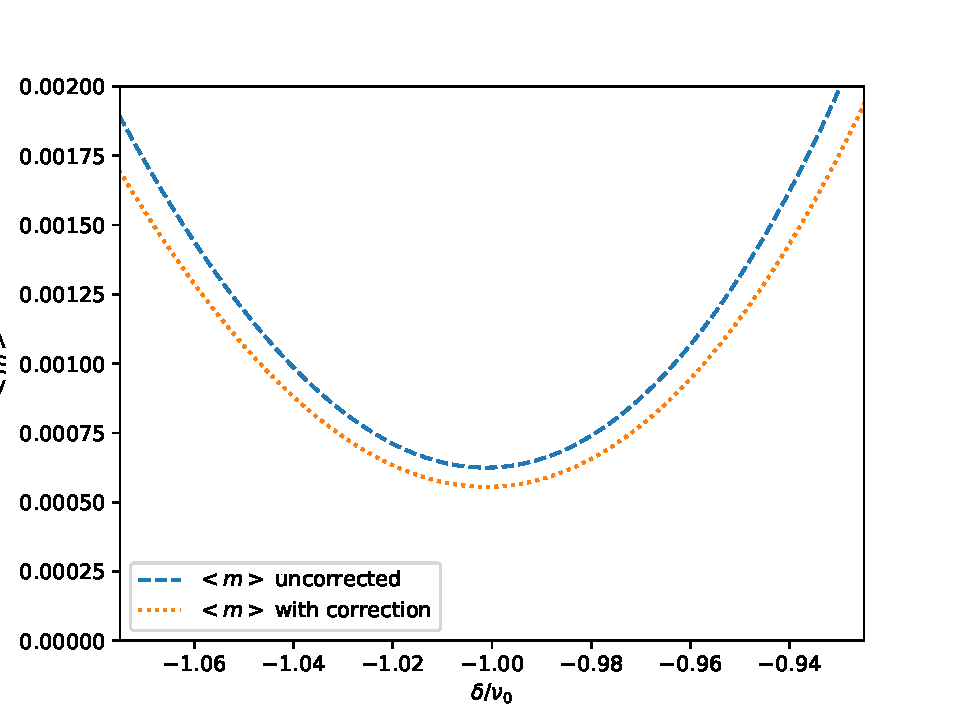
\includegraphics[scale=.5]{TempGorden1.pdf}   
\caption{ Mechanical oscillator phonon number with and without a time dependence. The correction results in a lower minimum temperature, as well as a lower temperature in a region around this minimum.}\label{fig:TempComparisson}
\end{figure}


\fxnote{Como acordamos por telefono: agrega una figura alrededor de
  $\delta=1$ y explica las dos figuras en el texto}

For figure \ref{fig:TempComparisson},we used $\kappa = 0.05\nu_0$ and
calculated $\expval{m}$ in the region
$\frac{\delta}{\nu_0}\in [-2,2]$. We restrict the figures to the
region near the temperature minimum at $\frac{\delta}{\nu_0}=-1$ The
positive half of the region corresponds to heating of the resonator
and the negative part corresponds to cooling. We assume that the
parameters are such that

\begin{equation}
\frac{C_tJ_1(C_t)}{I_0(C_t)} = 0.05,
\end{equation}
so that corrections proportional to higher orders in $C_t$ could be
disregarded. As we can see in figure \ref{fig:TempRatio}, the
corrected temperature is lower over a range around the minimum point.

It must be noted that since terms of order $\frac{\delta_t}{\delta^2}$
are neglected, the approximation does not hold as $\delta$ approaches
0. The approximation is valid near $\frac{\delta}{\nu_0} = -1$ as long
as $|\frac{\delta_t}{\nu_0}|,\frac{\delta_t}{\delta^2}\ll 1$. 

\begin{figure}
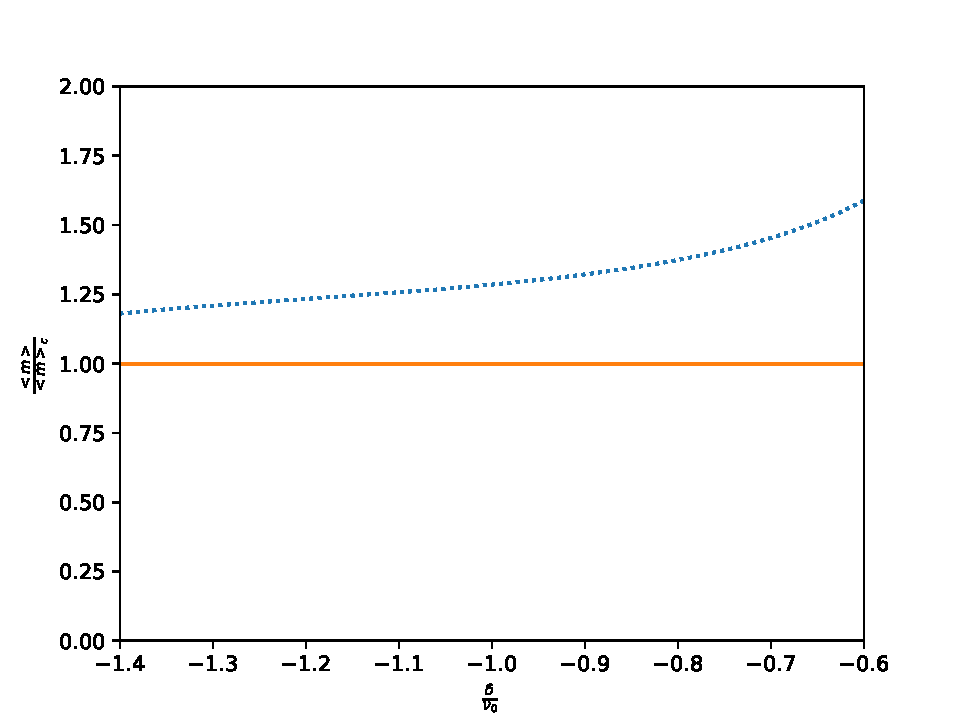
\includegraphics[scale=.5]{TempPropGorden1.pdf}
\caption{Ratio of the uncorrected and corrected temperatures over the cooling side of the detuning range. The corrected temperature is lower than the uncorrected temperature not just near the minimum.}
\label{fig:TempRatio}
\end{figure}




\section{Conclusions}\label{ConCl}

Using an improved theoretical description for the dissipation of a
parametrically driven mechanical object in an optomechanical setup, we
found that the lowest temperature reached can be lower than in the
non-driven case. This implies that periodically changing the natural
frequency of the mechanical object in optomechanics can be used for
reaching lower temperatures. This also opens the path for exploring
what happens if the movement of a leaky cavity is taken into
consideration when theoretically treating the dissipation of the
cavity field, because, similarly to the setup study in this paper, the
natural frequency of the cavity field changes periodically with time,
in addition to the time dependency the cavity acquires from the
harmonic oscillator. We plan to explore this case in future work.
 
\appendix
\section{The Damping Basis}\label{App1}

Master equations of the type 

\begin{equation}
\dot{\rho} = \mathcal{L}_{cav} \rho = \frac{1}{i\hbar}[H,\rho]+L_a\rho, 
\end{equation} with

\begin{align}\label{EMField}
L_a \rho =& - \frac{\kappa}{2}(n_p+1)[a^\dagger a\rho + \rho a^\dagger a -2a\rho a^\dagger] \nonumber \\
 &- \frac{\kappa}{2}(n_p)[ aa^\dagger\rho + \rho  aa^\dagger -2a^\dagger\rho a]\, ,
\end{align}
and
\begin{equation}
  H=\hbar \omega_c \, a^\dagger a\, ,
\end{equation}
model the behavior of a bosonic field inside a one mode leaky cavity
with frequency $\omega_c$; the cavity is in contact with a thermal bath
characterized by $n_p$ thermal photons, the cavity damping is given by
$\kappa$ \cite{EnglertDB} and $a^\dagger$, $a$ are cavity photons
creation and anhilation operators. The density operator can be
expressed in a basis given by the right Lindblad superoperator's
eigenstates, ${\hat{\rho}_n^j}$,
$n=0,1,2,...\qquad j = 0,\pm 1, \pm 2,... $, where
\begin{equation}
L\hat{\rho}_n^j = \lambda_n^j\hat{\rho}_n^j\label{eq:eigen_damping}\, ,
\end{equation}
with
\begin{equation}
\lambda_n^j = ij\omega_c -\kappa[n + \frac{|j|}{2}]\, .
\end{equation}
The real part of these eigenvalues corresponds to the 
eigenvalues of the operator $L_a$. This basis is known as the damping
basis \cite{EnglertDB} and is given by
\begin{align}\label{DefDB}
\hat{\rho}_n^l=&a^{\dagger j}\frac{(-1)^n}{(n_p+1)^{j+1}}:L_n^l[\frac{a^\dagger a}{n_p+1}]e^{-[\frac{a^\dagger a}{n_p+1}]}:\quad j \geq 0, \\
\hat{\rho}_n^j=&\frac{(-1)^n}{(n_p+1)^{|j|+1}}:L_n^{|j|}[\frac{a^\dagger a}{n_p+1}]e^{-[\frac{a^\dagger a}{n_p+1}]}:a^{|j|}\quad l \leq 0.
\end{align}
The Lindblad operator is not hermitian and the left eigenstates must
be considered to find the coefficients of the density operator
expansion in the damping basis. These are the eigenstates of the
equation $\check{\rho}_n^jL = \lambda_n^j\check{\rho}_n^j$ they have
the same eigenvalues and are given by
\begin{align}\label{DefDBDual}
\check{\rho}_n^j=&(\frac{-n_p}{n_p+1})^n\frac{n!}{(n+j)!}:L_n^j[\frac{a^\dagger a}{n_p}]:a^{j}\quad j \geq 0, \\
\check{\rho}_n^j=&(\frac{-n_p}{n_p+1})^n\frac{n!}{(n+|j|)!}a^{\dagger|j|}:L_n^{|j|}[\frac{a^\dagger a}{n_p}]:\quad j \leq 0.
\end{align}

The left and right eigenstates are orthogonal under the product
\begin{equation}
(\hat{\rho}_n^j,\check{\rho}_{n'}^{j'})=Tr[\hat{\rho}_n^j\check{\rho}_{n'}^{j'}] = \delta_{n,n'}\delta_{j,j'},
\end{equation} and fulfill

\begin{equation}\label{DampingBasisCompleteness}
\sum_{\lambda} \hat{\rho}_\lambda \otimes \check{\rho}_\lambda = \mathbb{I},
\end{equation} where the sum is over all possible eigenvalues. An important case is a cavity at zero temperature, in this case the right states are \cite{EnglertDB}

\begin{align}\label{DefDBZero}
\hat{\rho}_n^j=&a^{\dagger j}(-1)^{a^\dagger a + n}\binom{n+j}{a^\dagger a+j} \quad j \geq 0, \\
\hat{\rho}_n^j=&(-1)^{a^\dagger a + n}\binom{n+|j|}{a^\dagger a+|j|}a^{|j|} \quad j < 0,
\end{align} and the left states are

\begin{align}\label{DefDBDualZero}
\check{\rho}_n^j=&\frac{n!}{(n+j)!}\binom{a^\dagger a}{n}a^j \quad j \geq 0, \\
\check{\rho}_n^j=&a^{\dagger|j|}\frac{n!}{(n+|j|)!}\binom{a^\dagger a}{n} \quad j < 0.
\end{align}

These states play an important part in the derivation of the master
equation of the cavity state in the adiabatic approximation.

When there is no damping ($\kappa=0$) the left and right eigenstates reduces to 

\begin{equation}
\hat{\rho}_{n}^{j}=\Ket{n+j}\Bra{n}=\check{\rho}_{n}^{\dagger j},
\end{equation}
with eigenvalues
\begin{equation}
\lambda_l = i j \nu_0\, ,
\end{equation}
$\Ket{n}$ is the number state of the harmonic oscillator, $j$ is an
integer satisfying $(n+j)>0$.


\section{Laser Cooling and Projection Operators}\label{CoolingAppendix}

\fxnote{Agregar una explicacion explicita de como haces los promedios en el tiempo}

In order to find the master equation
\eqref{eq:ProyectedMasterEqCooling} we begin with the equation based on the Hamiltonian \eqref{LCHamiltonian}
\begin{equation}\label{eq:master_no_mechanical_damping}
\dot{\rho}=(\mathcal{L}_0+\mathcal{L}_1)\rho\, ,
\end{equation}
where
\begin{align}
\mathcal{L}_0=& \mathcal{L}_{cav} + \mathcal{L}_{mec},\\
 =&(\frac{1}{i\hbar}[H_{\rm cav}(t),\bullet]+L_a) +(\frac{1}{i\hbar}[H_{\rm mec},\bullet]), \nonumber
\end{align}
gives the free dynamics 
and
\begin{equation}
\mathcal{L}_1 = \frac{1}{i\hbar}[H_{\rm int},\bullet],
\end{equation}
gives the field-mechanic oscillator interaction.

Equation \eqref{eq:master_no_mechanical_damping} is the same as
equation \eqref{LCMasterEq} without the mechanical damping, which
occurs on a slower time scale than the other processes and can be
incorporated after the adiabatic approximation. We employ projection
operators, like those in \cite{CarmichaelQO}, to separate the
evolution into different time scales and perform an adiabatic
approximation. The projection operator $P$ projects the state into a
slow-decaying evolution space whereas the projection operator $Q$
projects the system into a fast-decaying evolution space, they fulfill
the completeness relation
\begin{equation}
1 = P + Q,
\end{equation}
and have the properties
\begin{enumerate}

\item $ P\mathcal{L}_{0} = \mathcal{L}_{0}P = 0 $\qquad as P projects the state to the stationary subspace
\item $P\mathcal{L}_{1}P=0$ \qquad as the interaction does not couple states in P

\item $P^2 = P \quad Q^2 = Q$ \qquad as $P$ and $Q$ are projectors.
\end{enumerate}
In the decay picture the master equation is 
\begin{equation}
  \label{eq:master_decay_picture}
    \dot{\rho'} = \mathcal{L}'_1\rho'\, ,
\end{equation}
where
\begin{align*}
 \rho' =& e^{\int_0^t \mathcal{L}_0 dt'}\rho,\\
  \mathcal{L}_1' =& e^{-\int_0^t \mathcal{L}_0 dt'}\mathcal{L}_1e^{\int_0^t \mathcal{L}_0 dt'}.
\end{align*} or more explicitly

\begin{align}
\rho' =& e^{-\mathcal{L}_0t - \mathcal{L}_0^t(t)}\rho,\\
\mathcal{L}_1' =&e^{-\mathcal{L}_0t - \mathcal{L}_0^t(t)}\mathcal{L}_1' e^{\mathcal{L}_0t +\mathcal{L}_0^t(t)},
\end{align} where $\mathcal{L}_0$ refers to all of the non time-dependent eigenvalues and $\mathcal{L}_0^t=\frac{\delta_t}{\nu_0} \sin(\nu_0t)[a^\dagger a,\bullet]$ refers to the explicitly time dependent part of the cavity Hamiltonian.  The time integration is needed because the cavity detuning is explicitly time dependent. We project the master equation \eqref{eq:master_decay_picture} into
both $P$ and $Q$ to obtain the equations 
\begin{align*}
P\dot{\rho}' =& P\mathcal{L}_1'Q\rho', \\
Q\dot{\rho}' =& Q\mathcal{L}'_1Q\rho' + Q\mathcal{L}'_1P\rho'.
\end{align*} The equation for $Q$ can be formally integrated

\begin{align*}
Q\rho =& Q\rho'(t_0) + \int_{t_0}^{t}dt' Q\mathcal{L}'_1(t')P\rho'(t')\\
       &+\int_{t_0}^{t}dt'Q\mathcal{L}'_1(t')Q\rho'(t'),
\end{align*}
 and then the Markov approximation is performed, approximating $\rho(t')$ by $\rho(t_0)$
\begin{align*}
Q\rho\simeq & Q\rho'(t_0) + \int_{t_0}^{t}dt' Q\mathcal{L}'_1(t')P\rho'(t_0)\\
       &+\int_{t_0}^{t}dt'Q\mathcal{L}'_1(t')Q\rho'(t_0),
\end{align*}
and this is substituted into the $P$ equation
\begin{align}
P\dot{\rho'}(t) =& P\mathcal{L}_1Q\rho'(t_0)\\ 
 &+ P\mathcal{L}_1\int_{t_0}^{t}dt' Q\mathcal{L}_1(t')P\rho'(t_0)\nonumber \\
 &+ P\mathcal{L}_1\int_{t_0}^{t}dt'Q\mathcal{L}_1(t')Q\rho'(t_0)\nonumber,
\end{align}
where only the second term is non zero as we can choose the initial condition to have no part in $Q$. We focus on this term and transform back from the decay
picture


\begin{align}\label{eq:temp_1}
P\dot{\rho}'(t)=&P e^{-\mathcal{L}_0 t-\mathcal{L}_0^t(t)}\mathcal{L}_1e^{\mathcal{L}_0 t+\mathcal{L}_0^t(t)}\\
\int_{t_0}^{t}dt'&Qe^{-\mathcal{L}_0 t'-\mathcal{L}_0^t(t')}\mathcal{L}_1e^{\mathcal{L}_0 t'+\mathcal{L}_0^t(t')}Pe^{-\mathcal{L}_0(t_0)-\mathcal{L}_0^t(t_0)}\rho(t_0).\nonumber
\end{align} We write the projectors as
\begin{eqnarray}
  P &=& \sum_{\lambda} (\hat{\rho}_{\lambda}^{cav}\otimes\hat{\rho}_{\lambda}^{mec})\otimes(\check{\rho}_{\lambda}^{cav}\otimes\check{\rho}_{\lambda}^{mec}),\label{eq:projector_p}\\
  Q &=& \sum_{\lambda'} (\hat{\rho}_{\lambda'}^{cav}\otimes \hat{\rho}_{\lambda'}^{mec})\otimes(\check{\rho}_{\lambda'}^{cav}\otimes\check{\rho}_{\lambda'}^{mec})\label{eq:projector_q}\, ,
\end{eqnarray}
the projectors with the $\lambda$ label project the state in the
slow-decaying time-scale subspace, they are eigenstates of
$\mathcal{L}_0+\mathcal{L}_0^t(t)$ with only zero eigenvalues. The projectors with the
$\lambda'$ label corresponds to the fast-decaying time-scale, they are
eigenstates of $\mathcal{L}_0+\mathcal{L}_0^t(t)$ with eigenvalues with a non-zero real
part, those states decay quickly. The projectors are applied via the product

\begin{equation}
PX =\sum_\lambda \hat{\rho_{\lambda}}Tr[\check{\rho}_{\lambda}X],
\end{equation} with

\begin{equation}
\hat{\rho}_\lambda = \hat{\rho}_\lambda^{mec} \otimes  \hat{\rho}_\lambda^{cav}.
\end{equation} We employ the states defined in Appendix
\ref{App1} for both the cavity and the mechanical resonator. 

Using equations \eqref{eq:projector_p} and \eqref{eq:projector_q} in
\eqref{eq:temp_1} and applying the operator $\mathcal{L}_0+\mathcal{L}_0^t(t)$ we obtain
\begin{align}\label{ProyectionEQ}
P\dot{\rho}'(t)=P e^{-\mathcal{L}_0 t-\mathcal{L}_0^t(t)}\mathcal{L}_1[&\sum_{\lambda',\lambda}\int_{t_0}^{t}dt'e^{\lambda' t} \hat{\rho}_{\lambda'} \otimes \check{\rho}_{\lambda'}e^{-\lambda' t'}\mathcal{L}_1\\
&e^{\lambda t'}\hat{\rho}_{\lambda} \otimes \check{\rho}_{\lambda} e^{-\lambda t_0}\rho(t_0)]\nonumber.
\end{align} where it is important to remember that the part of these eigenvalues that corresponds to the cavity has an explicitly time dependent part. To this effect, we split the eigenvalues into two distinct parts

\begin{align}
\lambda =& \lambda_0 + \lambda_c\frac{\delta_t}{\nu_0}\sin(\nu_0 t),\\
\lambda' =& \lambda'_0 + \lambda'_c\frac{\delta_t}{\nu_0}\sin(\nu_0 t),
\end{align}
as the time dependent part will be handled separately. $\lambda_c$
simply refers to \fxnote*{Sigue sin entenderse, ya que no dices quien es $i$, no se si lo que quieres decir es simplemente que $\lambda_c$ es igual a los enteros, y el valor depende simplemente sobre que estado actuo el operador L}{$i$ times the value acquired by the operator
$a^\dagger a$.} If we then set $t_0=0$ and note that
$\mathcal{L}_0^t(0)=0$, we may write \eqref{ProyectionEQ}, returning
$P$ and $Q$ to their original notation, as

\begin{align}
P\dot{\rho}'(t)=&\sum_{\lambda,\lambda'}[P \mathcal{L}_1Q[...]\mathcal{L}_1P\rho(0)],\\
[...] =& (\int_0^t dt' e^{(\lambda'_0-\lambda_0)t}e^{(\lambda_c'-\lambda_c)\frac{\delta_t}{\nu_0} \sin(\nu_0t)}e^{(\lambda_0-\lambda_0')t'}\nonumber \\ 
&\qquad \quad e^{(\lambda_c-\lambda_c')\frac{\delta_t}{\nu_0} \sin(\nu_0t')}),\nonumber
\end{align} In order to perform the integration we make the approximation
\begin{equation}
e^{(\lambda_c-\lambda_c')\frac{\delta_t}{\nu_0} \sin(\nu_0t')} \approx 1+(\lambda_c-\lambda_c')\frac{\delta_t}{\nu_0} \sin(\nu_0t'),
\end{equation} for the $t'$ term. This leads to

\begin{align}
&P\dot{\rho}'(t)\approx \\
&\sum_{\lambda'}P \mathcal{L}_1Q[\int_0^t dt' e^{(\lambda'_0-\lambda_0)t}e^{(\lambda_c'-\lambda_c)\frac{\delta_t}{\nu_0} \sin(\nu_0t)}e^{(\lambda_0-\lambda_0')t'}]\mathcal{L}_1P\rho(0)\nonumber \\
&+\frac{\delta_t}{\nu_0}\sum_{\lambda'}(\lambda_c-\lambda_c')P\mathcal{L}_1Q \nonumber\\
&[\int_0^t dt'\sin(\nu_0t') e^{(\lambda'_0-\lambda_0)t}e^{(\lambda_c'-\lambda_c)\frac{\delta_t}{\nu_0} \sin(\nu_0t)}e^{(\lambda_0-\lambda_0')t'}]\mathcal{L}_1P\rho(0),\nonumber
\end{align}

 After integration this results in

\begin{align}
P\dot{\rho}'(t)\approx& \sum_{\lambda'}P \mathcal{L}_1Q[E(\lambda')]\mathcal{L}_1P\rho(0)\\
&+\frac{\delta_t}{\nu_0}\sum_{\lambda'}P\mathcal{L}_1Q[E_c(\lambda')]\mathcal{L}_1P\rho(0),\nonumber
\end{align}  with

\begin{equation}
E(\lambda') = \frac{1}{-\lambda'_0}e^{\lambda_c'\frac{\delta_t}{\nu_0}\sin(\nu_0t)}.
\end{equation} and

\begin{equation}
E_c(\lambda')=\frac{(-\lambda'_c)((-\lambda'_0)\sin(\nu_0 t)-\nu_0\cos(\nu_0t))}{(-\lambda_0')^2 + \nu_0^2}e^{\lambda_c'\frac{\delta_t}{\nu_0}\sin(\nu_0t)}.
\end{equation} Here we have used the adiabatic approximation. For large enough $t$, $e^{\lambda'_0t}$ can be set equal to zero as the $\lambda'$ states decay very quickly.  We have also used that $\lambda$ states all have eigenvalues equal to zero. We then trace over all cavity degrees of freedom to obtain a master equation for the harmonic oscillator in the steady state subspace $P$. Here we assume that the initial condition is a separable state of the cavity and the harmonic oscillator $\rho(0)=\rho_{c}(0)\otimes\rho_{m}(0)$  and  set $\mu = Tr_c[P\rho_{cav}]$ to arrive at 

\begin{align}
\dot{\mu}=&\sum_{\lambda'}Tr_c[P \mathcal{L}_1Q[E(\lambda')]\mathcal{L}_1P\rho_{c}(0)\otimes\rho_{m}(0) ],\\
&+\sum_{\lambda'}\frac{\delta_t}{\nu_0}Tr_c[P\mathcal{L}_1Q[E_c(\lambda')]\mathcal{L}_1P\rho_{c}(0)\otimes\rho_{m}(0) ]\nonumber.
\end{align} we use the explicit form of $\mathcal{L}_1$ 

\begin{equation}
\mathcal{L}_1 = [\chi_0 F_aF_\Gamma,\cdot] = [\chi_0(\alpha_0 a^\dagger + \alpha_0^* a)(\gamma_-\Gamma^\dagger-\gamma_+\Gamma),\cdot],
\end{equation}and set $E= E(\lambda') +\frac{\delta_t}{\nu_0} E_c(\lambda')$ to  arrive at the expression

\begin{align*}
\dot{\mu} = \chi_0^2 \sum_{\lambda'}&( Tr_c[PF_aF_\Gamma QEF_aF_\Gamma \mu \otimes \rho_{c}]\\
&- Tr_c[PQEF_aF_\Gamma\mu \otimes \rho_{c} F_aF_\Gamma ]\nonumber \\
&-Tr_c[PF_aF_\Gamma QE\mu \otimes \rho_{c} F_aF_\Gamma ] \nonumber\\ 
&+Tr_c[PQE\mu \otimes \rho_{c}F_aF_\Gamma  F_aF_\Gamma ]). \nonumber
\end{align*}  We note that each projector is composed of a projector for cavity states and a projector for mechanical oscillator states, $P=P_c P_m$ so we can move everything that does not depend on the cavity outside of the trace to obtain

\begin{align}
\dot{\mu}=\chi_0^2 \sum_{\lambda'}& E(T_{1c}P_m[F_\Gamma,Q_m F_\Gamma \mu]\\
&-T_{2c}P_m[F_\Gamma,Q_m \mu F_\Gamma ]),\nonumber
\end{align} where $T_{1c}$ and $T_{2c}$ depend only on the cavity variables. These traces are readily calculated and result in

\begin{align}
T_{1c}=& Tr_c[F_aP_cF_a\rho_c]\\
=&\hbar^2\abs{\alpha_1}^2 \delta_{j,1}\delta{n,0},\\
T_{2c}=& Tr_c[F_aP_c\rho_cF_a]\\
=&\hbar^2 \abs{\alpha_1}^2 \delta_{j,-1}\delta{n,0},\\
\end{align} while the mechanical terms result in

\begin{align}\label{CoolingBeforecoefficients}
P_m[F_\Gamma,Q_m F_\Gamma \mu] =& \abs{\gamma}^2((\Gamma\Gamma^\dagger \mu - \Gamma^\dagger \mu  \Gamma)\delta_{l,-1} \\
&+ (\Gamma^\dagger\Gamma \mu - \Gamma \mu  \Gamma^\dagger)\delta_{l,1}),\nonumber \\
P_m[F_\Gamma,Q_m  \mu F_\Gamma] =& \abs{\gamma}^2((\Gamma\mu\Gamma^\dagger  - \mu\Gamma^\dagger   \Gamma)\delta_{l,-1}\\ 
&+ (\Gamma^\dagger \mu\Gamma -  \mu \Gamma \Gamma^\dagger)\delta_{l,1}). \nonumber
\end{align} the Kronecker deltas refer to the numbers in the eigenvalues, both for the cavity and the mechanical oscillator. These eliminate the sum over all possible $\lambda'$ values. This eigenvalue selection then determines the value of the functions $E(\lambda')$ and $E_c(\lambda')$ which are then averaged over time and equation \eqref{CoolingBeforecoefficients} can then be straightforwardly arranged in the form \eqref{eq:ProyectedMasterEqCooling}.

\bibliographystyle{unsrt}
\bibliography{Bib}
\end{document}